\section{Introduction}
I'm very glad to present by this report, my own project for Electronics for Embedded Systems course. The main idea consists in  realizing a camera able to capture photos to be transferred to an host computer for further processing. Before describing in details the environmental structure, I guess it's fundamental to highlight that all the topics of the course have been covered in the following manner:
\begin{itemize}
\item \textbf{Memory}: memory controller as FSM
\item \textbf{Programmable logic device}: acts as remote to send the user command
\item \textbf{Interconnection protocol}: I2C, SCCB and UART
\item \textbf{Peripheral management}: programming of camera peripheral
\item \textbf{AD and DA converters}: usage of AD converter to sample the luminance of the environment
\item \textbf{Power management}: Step-down converter to drive a LED
\end{itemize}
Each of them owns a proper section below.
Let's have a look on the general architecture, listing the main parts of the system. The camera is connected to an ST microcontroller: a STM32F446ZET. The choice on this MCU has due to the fact that it integrates a very useful and widespread engaged peripheral in the video-capturing field: the Digital CaMera Interface (\textbf{DCMI}). All images are sent to the host computer by UART protocol, exploiting another embedded peripheral of the microcontroller. Computer reads UART's data plugging a USB-UART adapter.  Then a small Python script converts those data into a BMP image. 
The command is generated by the user pushing a specific button. An 8 buttons keyboard is tied up to the FPGA: an Altera Cyclone IV on DE0-Nano board. The implemented VHDL is composed of the keyboard driver and a fully structural UART peripheral. When a button has clicked, an encoded 8-bit data is sent to the microcontroller, which, by an interrupt, recognizes that the user pushed something. 
A breadboard has been used to build circuits for AD and Bulk converters. 
I used STM32 CubeIDE to program the microcontroller , a software Eclipse based. To program the FPGA I exploited both Quartus II when uploading the \textit{sof} file and Xilinx ISE Design Suite when simulating (just for my high familiarity with that). Moreover, as classical laboratory instruments I relied on an oscilloscope provided by GW Instek and a multimeter for resistor measurements.
Moreover, I exploited the functionalities offered by GitHub, more specifically the desktop version that I found very easy and immediate to use.
\begin{figure}[H]
\centering

\includegraphics[scale=.5]{Immagini/03}
\end{figure}
For sure, the following image is more clarifying for the reader.

\begin{figure}[H]
\centering
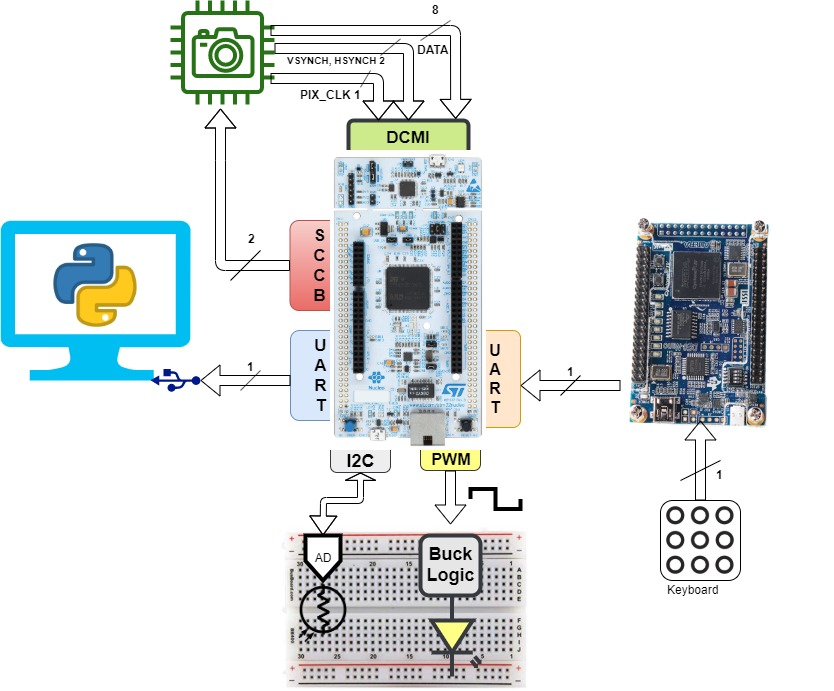
\includegraphics[scale=.5]{Immagini/01}
\label{01}
\caption{General block schema}
\end{figure}
Camera has been set to capture images in format QVGA (320x240) RGB 565 for an amount of 153600 bytes. However due to the poorness of memory  availability, I capture the half of them. Then the Python script generates on the host a picture 640x120 without colors.
\begin{figure}[H]
\centering
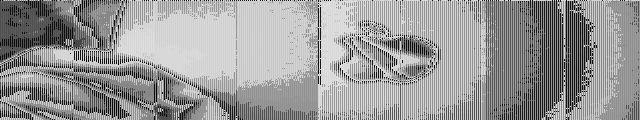
\includegraphics[scale=.04]{Immagini/04}
\label{04}
\caption{Apple logo captured by camera and then processed by software}
\end{figure}

\begin{figure}[H]
\centering
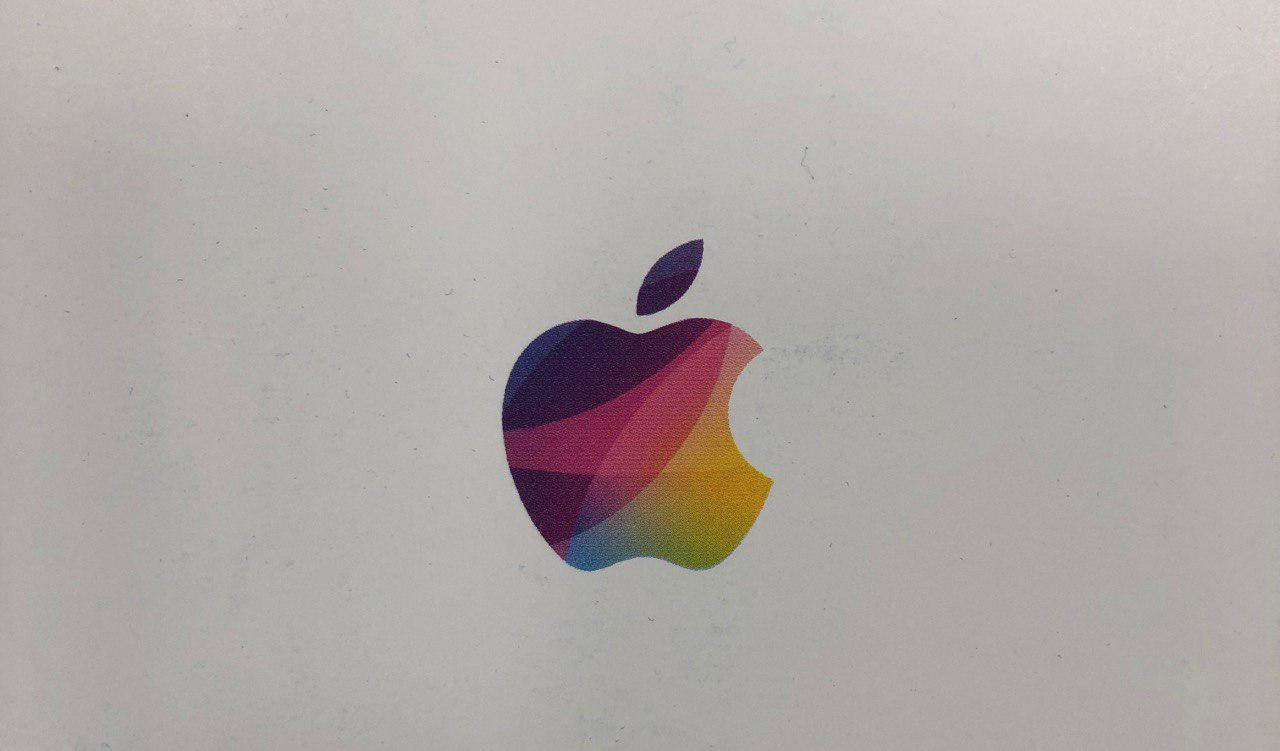
\includegraphics[scale=.1]{Immagini/05}
\label{05}
\caption{Original Apple logo}
\end{figure}
What actually the system appears\dots. It's a little bit messy due to the high number of flying wires. Only the camera requires 18 links.

\begin{figure}[H]
\centering
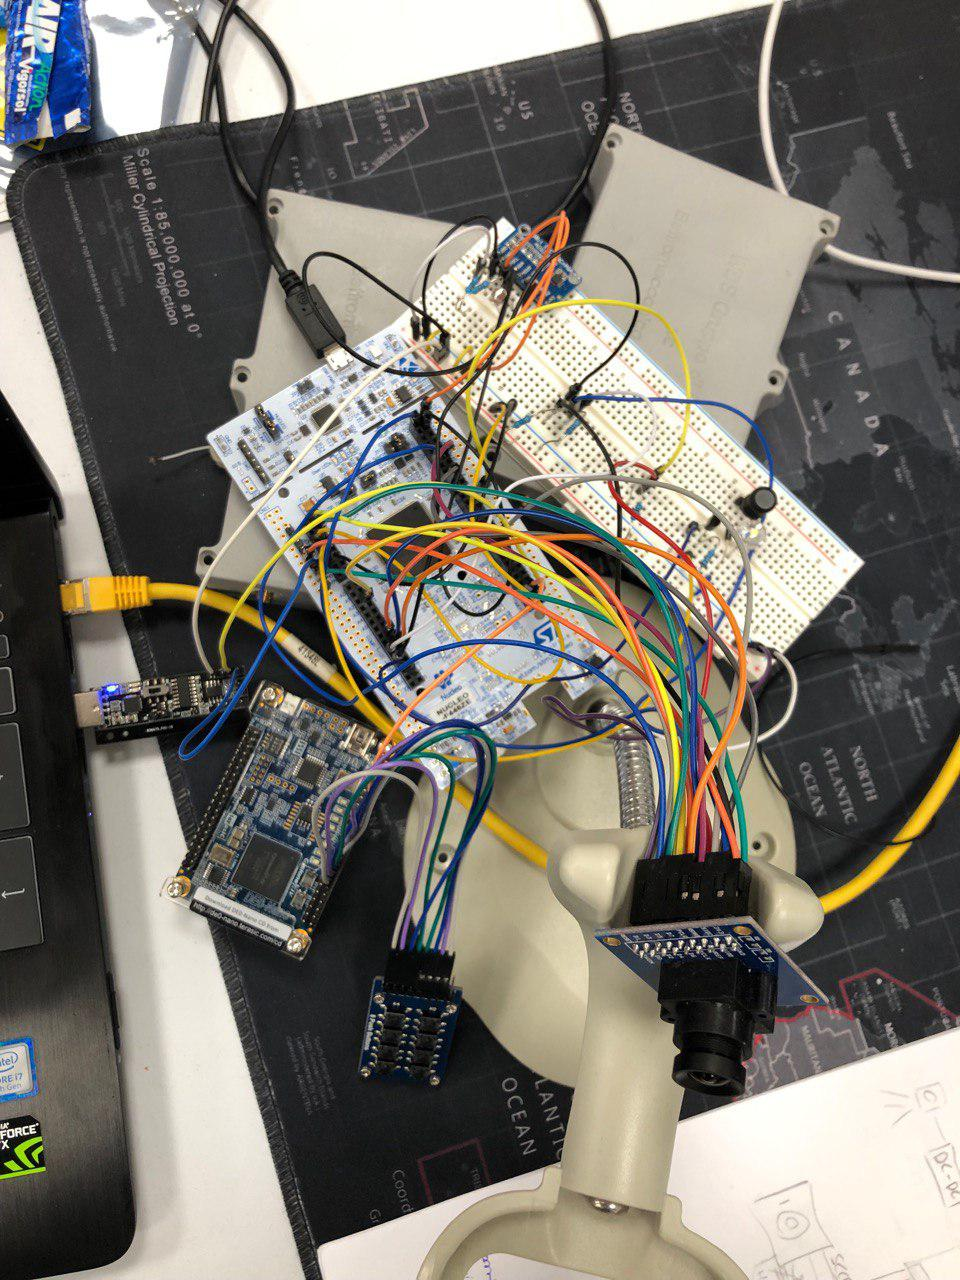
\includegraphics[scale=.4]{Immagini/02}
\label{02}
\caption{Real system}
\end{figure}

I'll proceed in the description in the same order I implemented each part of the project.